\documentclass[lettersize,journal]{IEEEtran}

\usepackage[utf8]{inputenc}
\usepackage{lmodern}
\usepackage[T1]{fontenc}
\usepackage[catalan]{babel}
\usepackage{mathtools}
\usepackage{float}
\usepackage{csvsimple}
\providecommand{\abs}[1]{\lvert#1\rvert}
\usepackage{braket}
\providecommand{\eq}[2]{
    \begin{equation}
        #2
    \label{eq:#1}
    \end{equation}
}
\usepackage{amsmath}
\DeclareMathOperator{\calA}{\mathcal{A}}
\DeclareMathOperator{\calH}{\mathcal{H}}
\DeclareMathOperator{\tr}{tr}
\usepackage{fancyhdr}
\usepackage{authblk}
\usepackage{abstract}
\usepackage{wrapfig}
\usepackage{graphicx}

\usepackage[backend=biber,style=phys]{biblatex}
\addbibresource{../TFG.bib}

% \usepackage{multirow}
% \usepackage[table,xcdraw]{xcolor}

% \usepackage{graphicx}
% \usepackage{caption}
% \usepackage{subcaption}

% \usepackage[a4paper]{geometry}
% \geometry{top=3cm, bottom=3.3cm, left=3cm, right=3cm}


\title{Entropia d'Entrellaçament i Holografia}
\author{Ferran Rodríguez Mascaró}
\date{}

\begin{document}


\maketitle{}


% \twocolumn[
%     \begin{@twocolumnfalse}
%         \maketitle{}
%         \begin{abstract}
%         ...
%         \end{abstract}
%     \end{@twocolumnfalse}
% ]

% \section{Introduction}
\section{Introducció}


% \subsection{Anti-de Sitter space-times}
\subsection{Espaitemps d'Anti-de Sitter}

% An anti-de Sitter (AdS) space-time is a maximally symmetric spacetime with negative curvature, solution to Einstein's equations with a negative cosmological constant.
Un espaitemps d'anti-de Sitter (AdS) és un espaitemps maximalment simètric amb curvatura negatica, solució de les equacions d'Einstein amb constant cosmològica negativa.

% A maximally symmetric spacetime with negative curvature, solution to Einstein's equations with a negative cosmological constant, is called an anti-de Sitter (AdS) spacetime.

% Its Riemann tensor is expressed as
% \begin{equation}
%     R_{abcd} = - \frac{1}{L^2} ( g_{ac} g_{bd} - g_{ad} g_{bc} ) ,
% \label{eq:AdS_Riemann}
% \end{equation}
% One can find that for these type of space-times to be solution of Einstein equations, the cosmological constant must be
% \begin{equation}
%     \Lambda = - \frac{(D-1)(D-2)}{2L^2} .
% \label{eq:AdS_cosmo-const}
% \end{equation}

% One can obtain the metric of the half-space of an AdS spacetime of $D=d+1$ dimensions using the coordinate system of the Pointcaré patch as
Es pot obtenir la mètrica del 'mig-espai' d'un espaitemps d'AdS de $D=d+1$ dimensions utilitzant les coordenades del 'Pointcaré patch' com
\eq{AdS_PP-metric}{
    ds_{AdS_D}^2 = \frac{1}{z^2} \left( -dt^2 + dz^2 + \sum_{i=1}^{d-1} dx_i^2 \right) \ ,
}
% with the time and space-related dimensions $t , x_i \in (-\infty,+\infty)$ and an extra dimension $z \in (0,+\infty)$ \cite{kaplan_lectures_nodate}.
amb les dimensions relacionades amb el temps i l'espai $t , x_i \in (-\infty,+\infty)$ i una dimensió extra $z \in (0,+\infty)$ \cite{kaplan_lectures_nodate}.

% Fixing the coordinate $z$, one creates $d$-dimensional Minkowski space-time surfaces 'weighted' by the factor $\frac{1}{z^2}$.
Fixant la coordenada $z$, es creen espaitemps de Minkowski $d$-dimensionals amb un factor de pes $\frac{1}{z^2}$.

\begin{wrapfigure}{r}{0.27\textwidth}
    \centering
    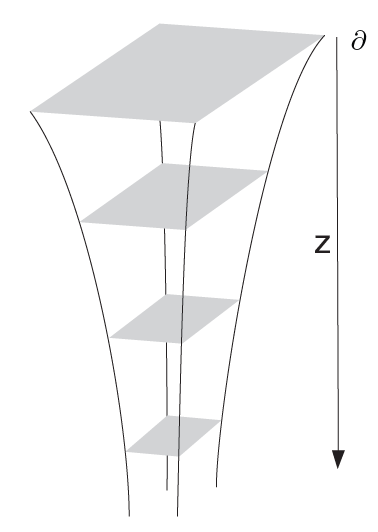
\includegraphics[width=0.15\textwidth]{../../Imatges/Captura_Superficies_z.png}
\caption{Representation of the different Minkowski space-time layers along the $z$ coordinate inside an AdS space-time.}
\label{fig:AdS_z-surfaces}
\end{wrapfigure}

% At constant time, \cite{} this metric forms hyperbolic spaces of negative curvature, conformally equivalent to Minkowski space-times at $z \to 0$. The conformal infinity of AdS is timelike, thus one needs boundary conditions to determine the future evolution uniquely.
% \footnotetext{A conformal or angle-preserving function is the one that preserves angles between curves at a certain point, as well as preserving orientation \cite{}.}
A temps constant, \cite{} aquesta mètrica forma spais hiperbòlics de curvatura negativa, conformalment equivalents a espaitemps de Minkowski per $z \to 0$. L'inifinit conforme d'AdS és de tipus temps, fent que es necessitin condicions de frontera per determinar l'evolució temporal unívocament.

% Using hyper-polar coordinates one can obtain a different expression for the metric which covers the entire space:
Utilitzant coordenades hiperpolars s'obté una altre expressió per a la mètrica que cobreix tot l'espai:
\eq{AdS_hyper-polar-metric}{
    ds_{AdS_D}^2 = \left [ - \left ( 1 + \frac{r^2}{L^2} \right ) dt^2 + \frac{dr^2}{\left ( 1+ \frac{r^2}{L^2} \right )} + r^2 d \Omega_{D-2}^2 \right ] \ ,
}
% being $L$ ($k^2=1/L^2$) the so called anti-de Sitter radius.
sent $L$ ($k^2=1/L^2$) l'anomenat radi d'anti-de Sitter.

\begin{wrapfigure}{r}{0.27\textwidth}
    \centering
    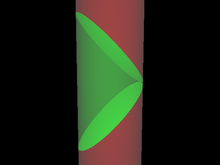
\includegraphics[width=0.21\textwidth]{../../Imatges/Wikipedia_Half-space_Cilindric.png}
% \caption{Representation of the half-space region of an AdS space-time and its boundary.}
\caption{Representació de la regió de 'mig-espai' d'un espaitemps d'AdS i la seva frontera.}
\label{fig:AdS_cylindrical}
\end{wrapfigure}

% In Figure \ref{fig:AdS_cylindrical} it is represented the metric of Equation \ref{eq:AdS_hyper-polar-metric}. The whole cylinder corresponds to an AdS space-time, being the lateral surface the conformal boundary (where $z \to 0$, or $r \to \infty$). The marked region corresponds to the one covered by the half-space coordinates, flanked by the conformal boundary and two lightlike geodesic hyperplanes \cite{}.
A la figura \ref{fig:AdS_cylindrical} s'hi representa la mètrica de l'Equació \ref{eq:AdS_hyper-polar-metric}. El cilíndre sencer correspón a un espaitemps d'AdS, sent la superfície lateral la frontera conforme (on $z \to 0$, o $r \to \infty$). La regió remarcada correspon a la que cobreixen les coordenades del 'mig-espai', envoltades per la forntera conforme i dos hiperplans geodèsics de tipus llum \cite{}.


% \subsection{Conformal Field Theories}
\subsection{Teories de Camps Conforme}

% A conformal field theory (CFT) is a quantum field theory that is invariant under transformations that locally preserve angles.
Una teoria de camps conforme (CFT) és una teoria quàntica de camps que és invariant sota transformacions que preserven localment els angles.


% \subsection{The Holographic Principle}
\subsection{El Principi Hologràfic}

% The covariant entropy bound \cite{bousso_covariant_1999} is conjectured as the representation of the universal law, in a four-dimensional space-time on which Einstein’s equation is satisfied, in which the entropy of a system is bounded by its area. It says that the number of independent degrees of freedom on any light-sheet of a surface cannot exceed a quarter of the area of this surfaces.
El límit de l'entropia covariant \cite{bousso_covariant_1999} és conjectura com a representació de la llei universal en la que, en un espaitemps de quatre dimensions en el què es satisfan les equacions d'Einstein, l'entropia d'un sistema està limitat per la seva àrea.

% This bound implies that the degrees of freedom inside some region grows with the area of the boundary and not as the volume of the region. This behavior leads to the \textit{holographic principle}, wich states that in a quantum gravity theory all the physics phenomena within some volume can be described in terms of a theory on the boundary of the area of the volume, which has less than one degree of freedom per Planck area \cite{t_hooft_dimensional_2009}.
Aquest límit impica que els graus de llibertat dins una regió creix segons l'àrea de la frontera i no segons el volum de la regió. Aquest comportament porta al \textit{principi hologràfic}, que diu que en una teoria de gravitació quàntica tots els fenòmens físics dins d'un volum es poden descriure en termes d'una teoria a la frontera de l'àrea del volum, el qual té menys d'un grau de llibertat per àrea de Planck \cite{t_hooft_dimensional_2009}.


% \subsection{AdS/CFT Correspondance}
\subsection{Correspondència AdS/CFT}

% A class of conformal field theories are equivalently described in certain limits in terms of anti-de Sitter space-times \cite{rangamani_holographic_2017}.
Un tipus de teoria de camps conforme és descriu equivalentment en certs límits en termes d'un espaitemps d'anti-de Sitter \cite{rangamani_holographic_2017}.

% The \textit{AdS/CFT Correspondance}, simply called \textit{holography} in high energy physics, is an equivalence or duality between quantum gravity theories (certain string theories) at asymptotically $D$-dimensional anti-de Sitter space-times and non-gravitational conformal quantum field theories at Minkowski space-times of $D-1$ dimensions \cite{maldacena_large_1999}. It allows us to study different aspects of each of these theories through the other. The so called \textit{holographic dictionary} relates quantities (observables) between the AdS theories and the CFT. % \cite{kaplan_lectures_nodate}
La \textit{correspondència AdS/CFT}, anomenada simplement \textit{holografia} a física d'altes energies, és una equivalència o dualitat entre teories de gravetat quàntica (certes teories de cordes) asimptòticament a espaitemps d'anti-de Sitter $D$-dimensionals i teories de camps conformes no gravitacionals de $D-1$ dimensions \cite{maldacena_large_1999}. Permet estudiar diferents aspectes de cada teoria a través de l'altre. L'anomenat \textit{diccionari hologràfic} relaciona quantitats (observables) entre les teories d'AdS i les CFT.


% \subsection{Entanglement Entropy}
\subsection{Entropia d'Entrellaçament}

% When two quantum systems enter into temporary physical interaction, they can no longer be described in the same way after a time of mutual influence \cite{schrodinger_discussion_1935}. One can no longer describe neither of those systems independently without losing global information, because the state of each systems know is influenced and correlated by the other system. This is the so called \textit{quantum entanglement}.
Quan dos sistemes quàntics entren temporalment en interacció física, deixen de poder-se descriure de la mateixa manera després d'un cert temps d'influència mútua \cite{schrodinger_discussion_1935}. No es podran descriure cap dels dos sistemes per separat sense perdre informació global, ja que l'estat de cada sistema ara està influit i correlacionat per l'altre sistema. Aquest és l'anomenat \textit{entrellaçament quàntic}.

Being two quantum systems represented by the corresponding Hillberg spaces $\calH_A$ and $\calH_B$, and an state $\ket{\Psi} \in \calH = \calH_A \otimes \calH_B$, this would be an entangled state if
\eq{entanglement}{
    \ket{\Psi} \neq \ket{\Psi_A} \otimes \ket{\Psi_B} \ \longrightarrow \ \ket{\Psi} = \sum_{i,j} c_{ij} \ket{i}_A \otimes \ket{j}_B \ ,
}
being $\ket{\Psi_{A,B}}$ the possible different substates in which one could separate $\ket{\Psi}$ if it was separable, substates expressed in each orthonormal bases $\{ \ket{k}_{A,B} \}$ of $\calH_{A,B}$ \cite{}.

The \textit{entanglement entropy} is a measure of the degree of quantum entanglement between the two subsystems composing a full quantum system \cite{nishioka_entanglement_2018}. It is defined by the von
Neumann entropy of the reduced density matrix $\rho_A$ of one of the subsystems as
\eq{entanglement-entropy}{
    S_{EE}(A) = - \tr_A ( \rho_A \log \rho_A ) \ ,
}
being $\rho_A = \tr_B \ket{\Psi}\bra{\Psi}$. If $\rho_A$ is diagonalized ($\rho_A = \sum_i \lambda_i \ket{i}\bra{i}$), then the entanglement entropy would take the simplified form $S_{EE} = - \sum_i \lambda_i \log \lambda_i$.

If there is no entanglement between both subsystems, the entanglement entropy is null ($S_{EE} = 0$).


\subsection{Entanglement entropy in AdS/CFT}

\begin{wrapfigure}{r}{0.27\textwidth}
    \centering
    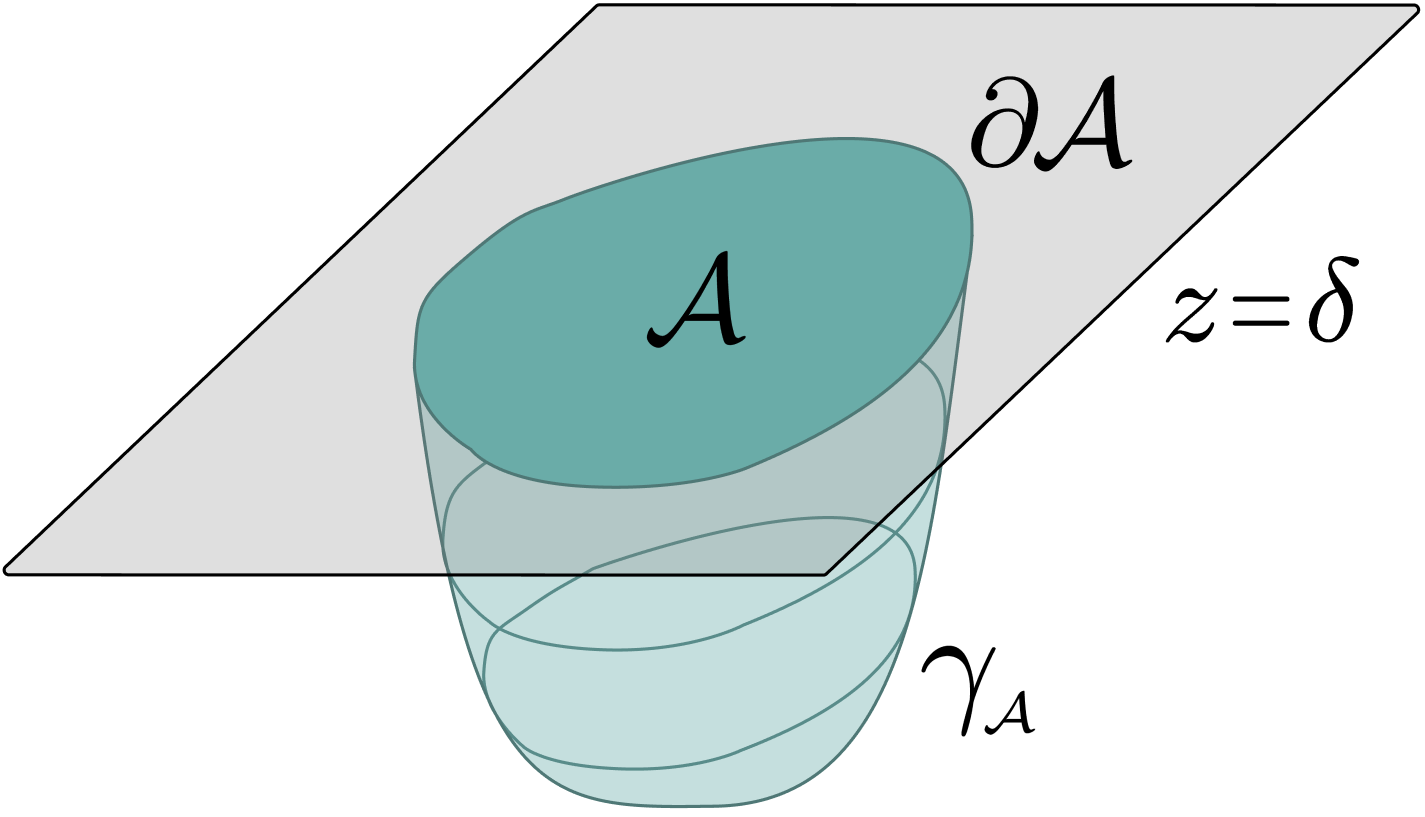
\includegraphics[width=0.27\textwidth]{../../Imatges/EE_AdS-CFT.png}
\caption{Region $\calA$ (dark blue) and its boundary $\partial \calA$ inside a $z=\delta$ AdS slide (grey) and its respective $\gamma_{\calA}$ (light blue) inside the AdS space-time.}
\label{fig:EE_AdS-CFT}
\end{wrapfigure}

In a quantum field placed in a Minkowski space-time, at a given time, every point on space is entangled with the points surrounding it \cite{nishioka_entanglement_2018}. Therefore, the entanglement entropy between a subsytem and the rest of the space will be dominated by the correlations between both sides of the boundary that isolates the subsystem.

% \begin{wrapfigure}{r}{0.25\textwidth}
%     \centering
%     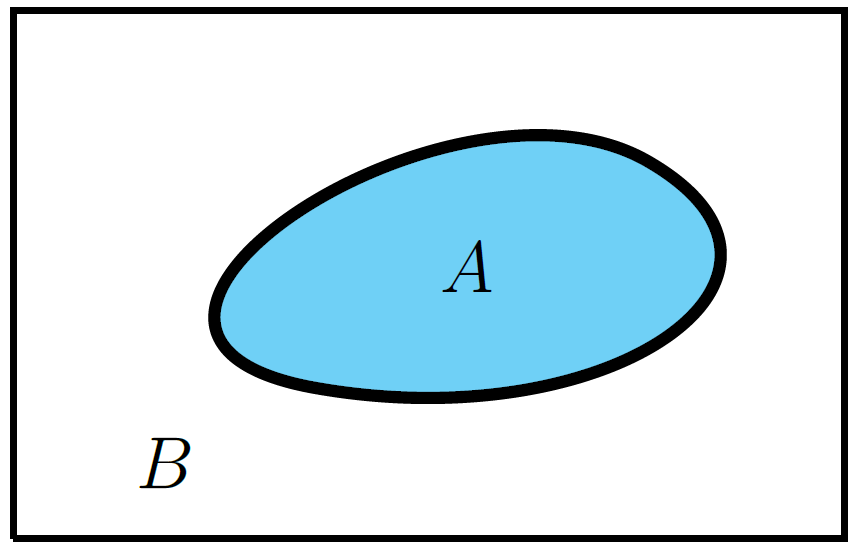
\includegraphics[width=0.24\textwidth]{../Imatges/Captura_EE_Frontera.png}
% \caption{Bipartion of a system in two complementary regions A and B.}
% \label{fig:EE_Minkowski-boundary}
% \end{wrapfigure}

% \begin{figure}[h!]
%     \centering
%     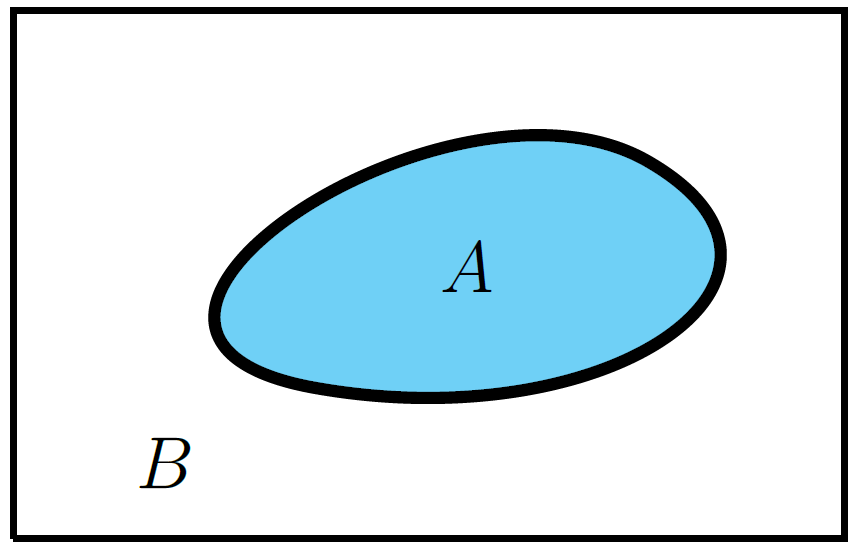
\includegraphics[scale=0.2]{../Imatges/Captura_EE_Frontera.png}
% \caption{Bipartion of a system in two complementary regions A and B.}
% \label{fig:EE_Minkowski-boundary}
% \end{figure}

In an ($d+1$)-dimensional AdS space-time, being $\calA$ a region of a $d$-dimensional Minkowski space-time slice formed from fixing $z$ as $z=\delta \ll 1$, the entanglement entropy of a $d$-dimensional CFT on this Minkowski space-time will be expressed by the so called Ryu-Takayanagi formula
\eq{EE_RT}{
    S_{\calA} = \frac{ \text{Area}(\gamma_{\calA}) }{ 4 G_{d+1} } \ ,
}
\cite{ryu_holographic_2008} where $\gamma_{\calA}$ is the surface of minimal area on the whole AdS space-time connected to the ($d-1$)-dimensional boundary $\partial \calA$ of the region $\calA$, and $G_{d+1}$ is the ($d+1$)-dimensional Newton constant (represented in Figure \ref{fig:EE_AdS-CFT}).

The area of $\gamma_{\calA}$ is obtained by
\eq{EE_RT-area}{
    \text{Area}(\gamma_{\calA}) = \int_{\gamma_{\calA}} \sqrt{h} \ d^{d}y \ ,
}
where $y$ are the $d$ coordinates that represent surface $\gamma_{\calA}$ and $h$ is the determinant of the metric $h_{ij} = \frac{\partial x^\mu}{\partial y^i} \frac{\partial x^\nu}{\partial y^j} g_{\mu\nu}$ induced on the surface by the surrounding space-time.

The Ryu-Takayanagi formula is valid for generic systems, and gives a flavour of how the geometry of space-time can emerge from mere quantum information. As a curiosity, the Ryu-Takayanagi formula in the case of a thermalized system of particles in an AdS space-time derives to the Bekenstein-Hawking formula \cite{bekenstein_black_1973} for the entropy a black hole:
\eq{BH}{
    S_{BH} = \frac{ A_H }{ 4 G } \ ,
}
that says that the entropy related to a black hole only depends on the area $A_H$ of its event horizon.

Solving the Ryu-Takayanagi formula for a ($d+1$)-dimensional anti-de Sitter space-time one obtains the expected general expression of the entanglement entropy for a $d$-dimensional quantum field theory:
\eq{EE}{
    S_{QFT_d} = \sum_{i=0}^{d/2-1} c_i \left( \frac{R}{\delta} \right) ^{d-2(i+1)} + a \log \left( \frac{R}{\delta} \right) - F \ ,
}
\cite{nishioka_entanglement_2018} in which $R$ is the characteristic length of the region studied, $c_i$ are coefficients that can be dependent on $\delta$, the logarithmic component only appears for even $d$, and $F$ is a function related to the aspect of the region $\calA$.


\printbibliography

\end{document}